\documentclass[aps,prb,nofootinbib,amsmath,amssymb,superscriptaddress,showpacs,twocolumn,floatfix]{revtex4-2}

\usepackage{graphicx}
%\usepackage{float}  		
\usepackage{url}
\usepackage{natbib}
%\usepackage{longtable}    
\usepackage{threeparttable}
\usepackage{booktabs}
\usepackage{multirow}
\usepackage{dcolumn}
\usepackage{bm}
\usepackage{color}
\usepackage{amsmath}
\usepackage{xfrac}
\usepackage{verbatim}
\usepackage{array}
\usepackage{chngcntr}
\usepackage{physics}
% \usepackage{notes2bib}
%\usepackage{caption}
%\usepackage{subcaption}
%\usepackage{ulem}
\usepackage[colorlinks,hyperindex]{hyperref}
	\hypersetup
		{colorlinks,	
	 	citecolor=blue,	
	 	linkcolor=blue,	
	 	urlcolor=blue,	
		}
%\graphicspath{{./fig/}} 	
\bibliographystyle{apsrev4-1}

\begin{document}
\title{Supplemental Material for Transferable Graph Neural Fingerprint Models for Quick Response to Future Bio-Threats}

%\author{Authors Anonymous}

\author{Wei Chen}
\thanks{Contributed equally to this work}
\affiliation{Center for Functional Nanomaterials, Brookhaven National Laboratory, Upton, New York 11973}

\author{Yihui Ren}
\thanks{Contributed equally to this work}
\affiliation{Computational Science Initiative, Brookhaven National Laboratory, Upton, New York 11973}

\author{Ai Kagawa}
\affiliation{Computational Science Initiative, Brookhaven National Laboratory, Upton, New York 11973}

\author{Matthew R. Carbone}
\affiliation{Computational Science Initiative, Brookhaven National Laboratory, Upton, New York 11973}

\author{Samuel Yen-Chi Chen}
\affiliation{Computational Science Initiative, Brookhaven National Laboratory, Upton, New York 11973}

\author{Xiaohui Qu}
\affiliation{Center for Functional Nanomaterials, Brookhaven National Laboratory, Upton, New York 11973}

\author{Shinjae Yoo}
\affiliation{Computational Science Initiative, Brookhaven National Laboratory, Upton, New York 11973}

\author{Austin Clyde}
\affiliation{Computational Science \& Data Science and Learning Division, Argonne National Laboratory, Lemont, Illinois 60439}

\author{Arvind Ramanathan}
\affiliation{Data Science and Learning Division, Argonne National Laboratory, Lemont, Illinois 60439}

\author{Rick L. Stevens}
\affiliation{Computing, Environment and Life Sciences, Argonne National Laboratory, Lemont, Illinois 60439}

\author{Hubertus J. J. van Dam}
\email{hvandam@bnl.gov}
\affiliation{Condensed Matter Physics and Materials Science, Brookhaven National Laboratory, Upton, New York 11973}

\author{Deyu Lu}
\email{dlu@bnl.gov}
\affiliation{Center for Functional Nanomaterials, Brookhaven National Laboratory, Upton, New York 11973}

\maketitle
\appendix

\setcounter{figure}{0}
\setcounter{table}{0}

\makeatletter 
\renewcommand{\thefigure}{S\@arabic\c@figure}
\renewcommand{\thetable}{S\@arabic\c@table}  
\makeatother

%\newpage
%\begin{center}
%Supplemental Materials: Predicting Ligand Docking Scores Using Graph Neural Fingerprints
%\end{center}

\section{GCN and GraphSAGE Model architectures}

\noindent
The node and edge embedding procedures map 
from vectors in the feature dimensions
to vectors in the embedding dimensions respectively for nodes and edges.  The node and edge feature and embedding dimensions are shown in the following tables.

\vspace{.3cm}

\begin{tabular}{|l|l|}
\hline
Node feature dimensions   & {[}11, 7, 9, 8, 6, 3{]}     \\ \hline
Node embedding dimensions & {[}15, 15, 15, 10, 10, 5{]} \\ \hline
\end{tabular}

\vspace{.3cm}

\begin{tabular}{|l|l|}
\hline
Edge feature dimensions   & {[}5, 5{]}   \\ \hline
Edge embedding dimensions & {[}35, 35{]} \\ \hline
\end{tabular}

\vspace{.3cm}
\noindent
The output of the universal neural fingerprint layers is the input of the fully connected, multilayer perceptron (MLP). 
This MLP consists of two layers, and the number of nodes in each layer
and activation functions are listed in the following tables.
ReLU is Rectified Linear Unit.

\vspace{.3cm}
\begin{tabular}{ | p{4.5cm} | p{3cm} | }%{|l|l|}
\hline
Number of nodes from inputs to outputs   
& {[} 70, 35, 1{]}  \\ \hline
Activation functions from the first layer to last layer 
& {[} ReLU, None {]}  \\ \hline
\end{tabular}

\section{Details on training the machine learning models}
The docking dataset was randomly split into 240,000, 30,000, and 30,457 samples for training, validation, and testing, respectively, using the \emph{numpy.random.shuffle} function~\cite{harris2020array}. The validation set was used to optimize hyperparameters including the numbers of hidden layers and neurons as well as perform early stopping (maximum 300 epochs) and model selection. The mean squared error (MSE) was used as the loss function. The models were trained using the ADAM optimizer~\cite{kingma2014adam} with batch size 64. The initial learning rate was 0.001 with a reducing factor of 0.7 and a minimum learning rate of $10^{-5}$. This ML experiments were conducted using one node of the BNL institutional cluster. Our code used 20 Intel Xeon Gold 6248 processors and a NVIDIA V100 GPU on one node of the cluster.  Each experiment for a particular target takes about 5-6 hours.

\begin{figure}
    \centering
    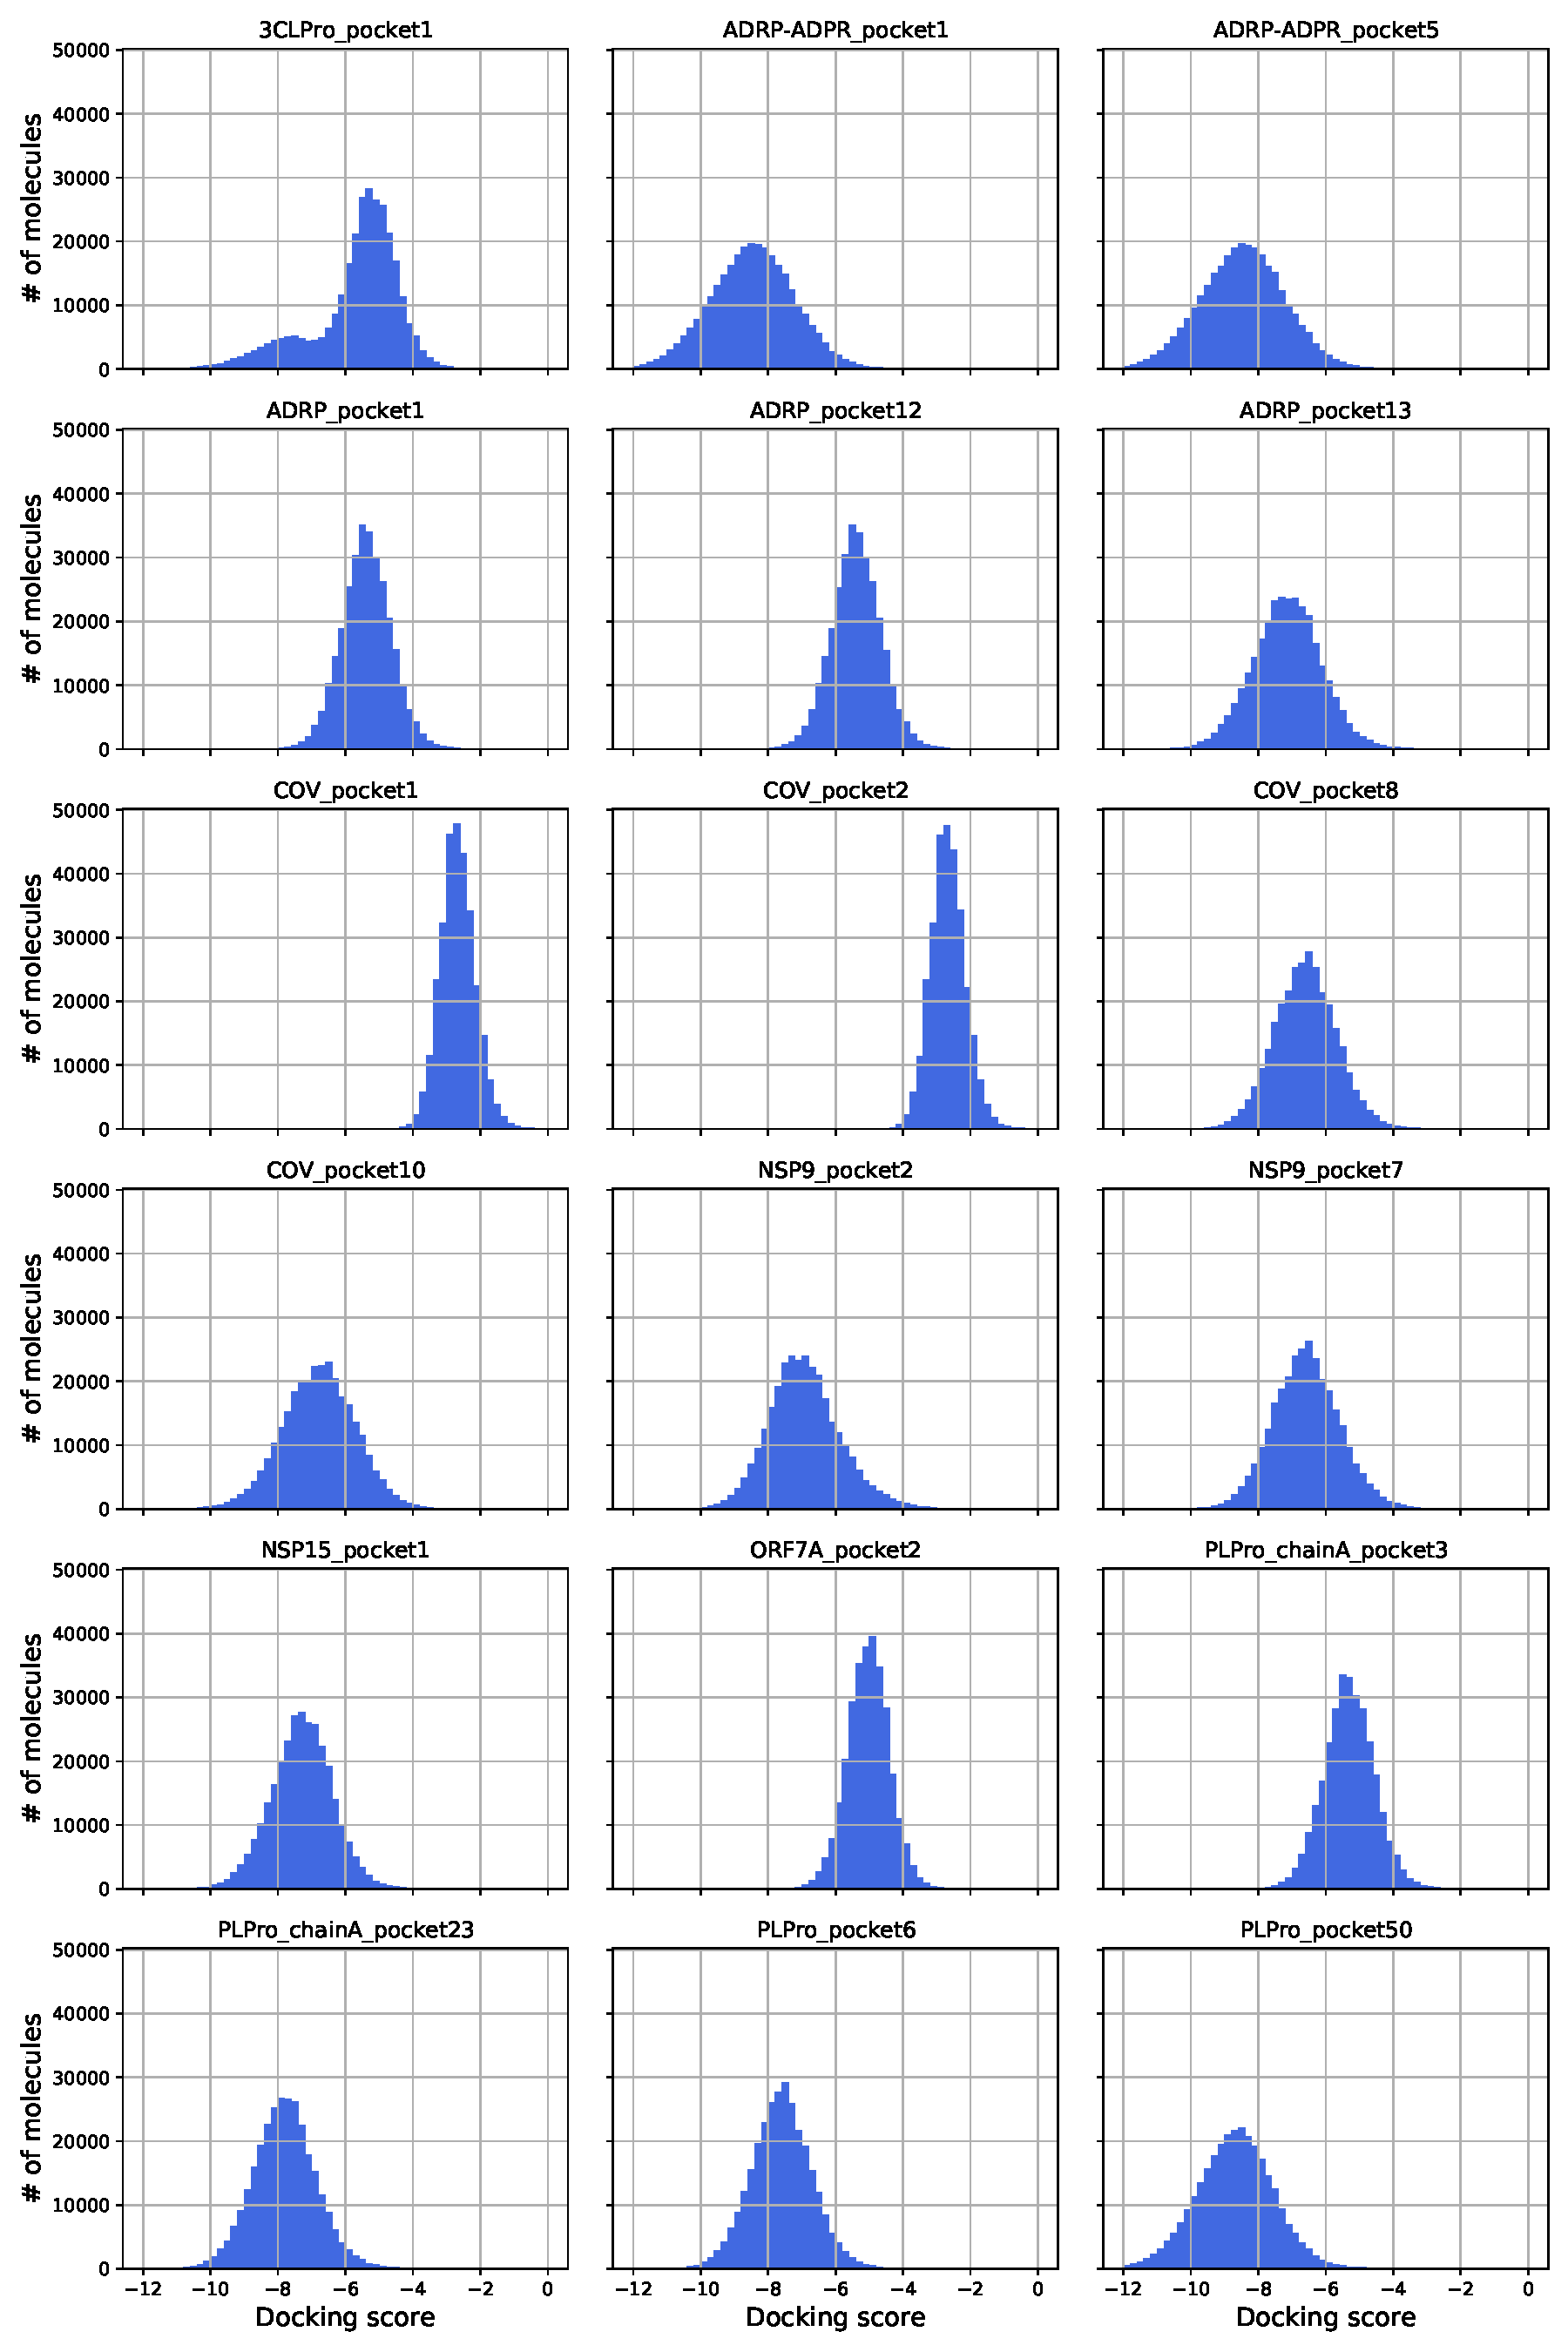
\includegraphics[width=0.9\hsize]{FigS1_score_hist.pdf}
    \caption{\label{fig_s:dist} Docking score distributions of molecules for 18 docking targets. The scores are in units of kcal/mol.
    }
\end{figure}

\begin{figure}
    \centering
    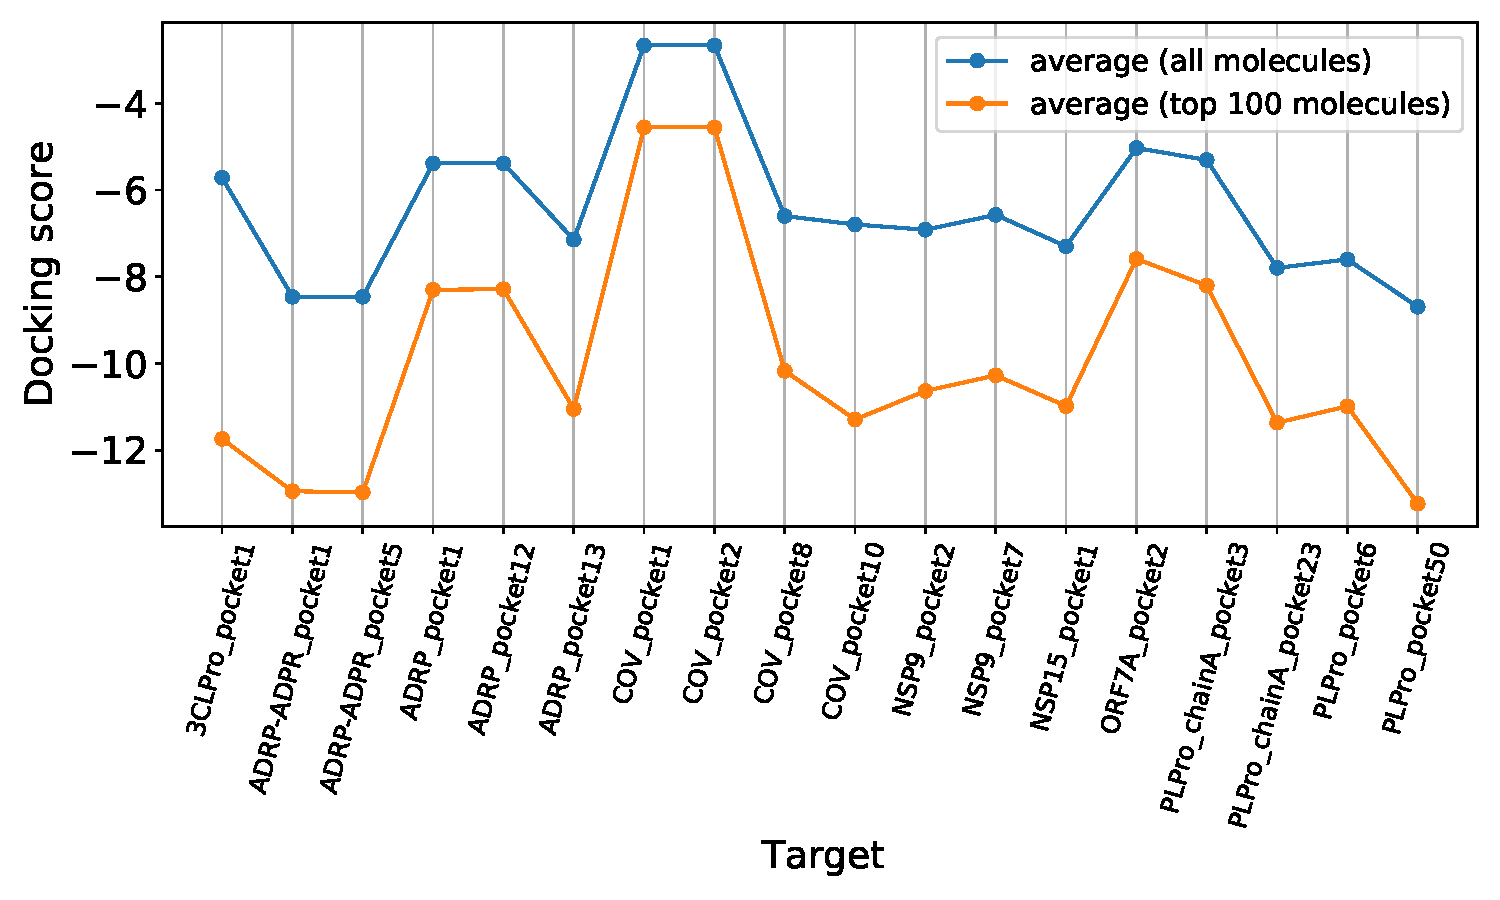
\includegraphics[width=\hsize]{FigS2_score_avg.pdf}
    \caption{\label{fig_s:avg} Average docking scores of molecules for 18 docking targets. 
    }
\end{figure}

\begin{figure}[b!]
    \centering
    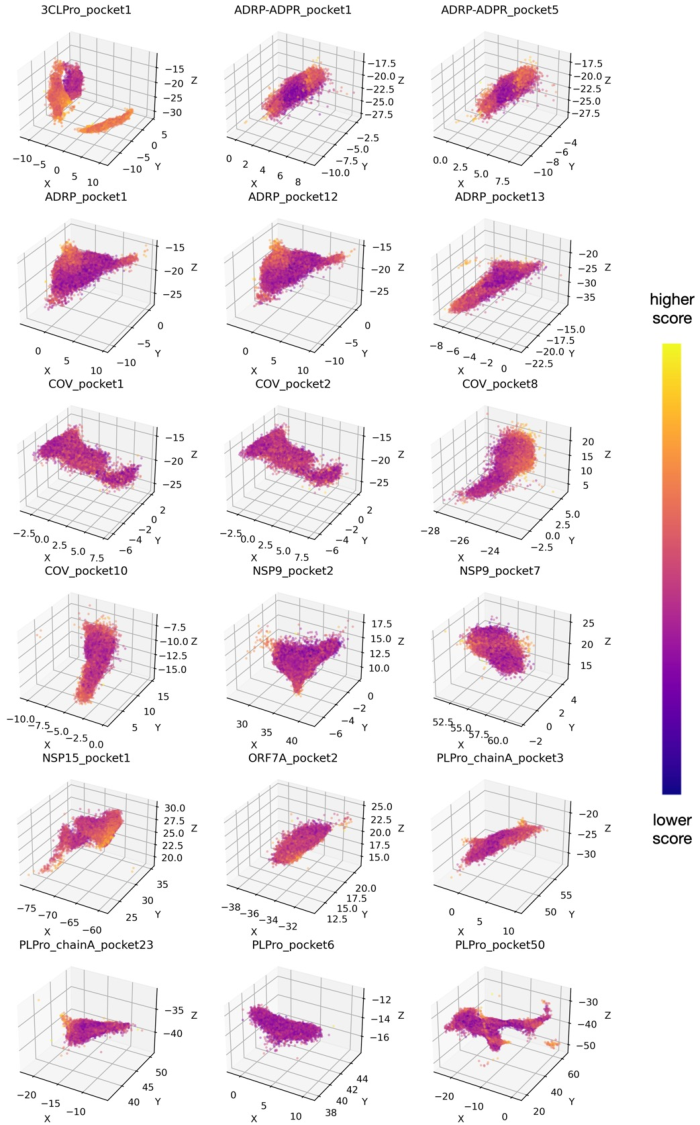
\includegraphics[width=\hsize]{FigS3_score_com.pdf}
    \caption{\label{fig_s:com} Center-of-mass distributions of molecules for 18 docking targets. The coordinates are in units of angstrom.
    }
\end{figure}

\begin{figure}[t!]
    \centering
    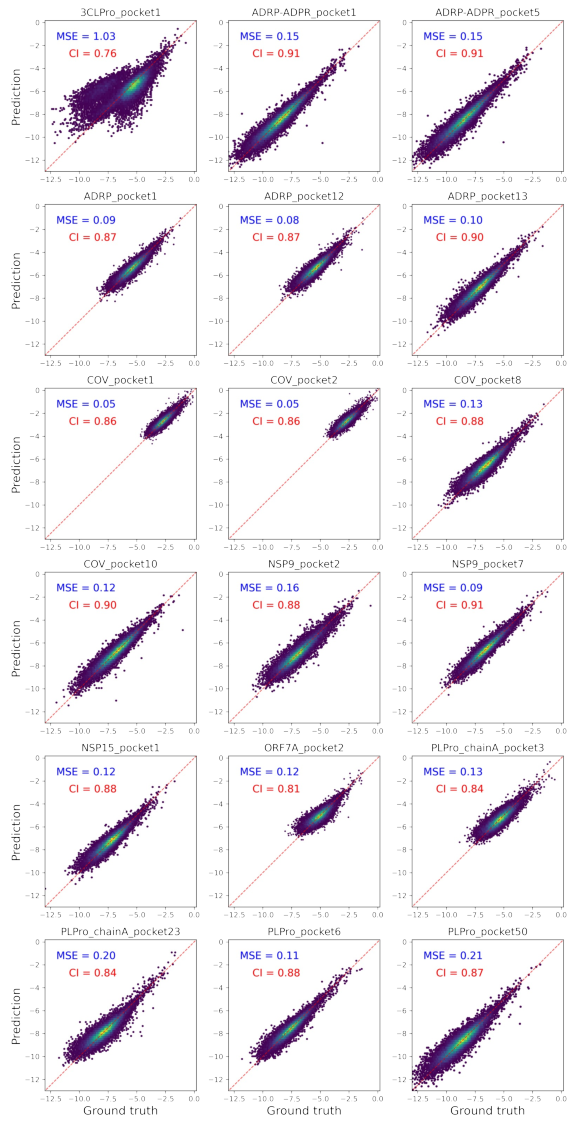
\includegraphics[width=0.9\hsize]{FigS4_single_model.pdf}
    \caption{\label{fig_s:mse} Prediction performance on the test sets by the GatedGCN model. MSE stands for mean squared error and CI for concordance index.
    }
\end{figure}

\vspace{\baselineskip}

\begin{figure}[ht]
    \centering
    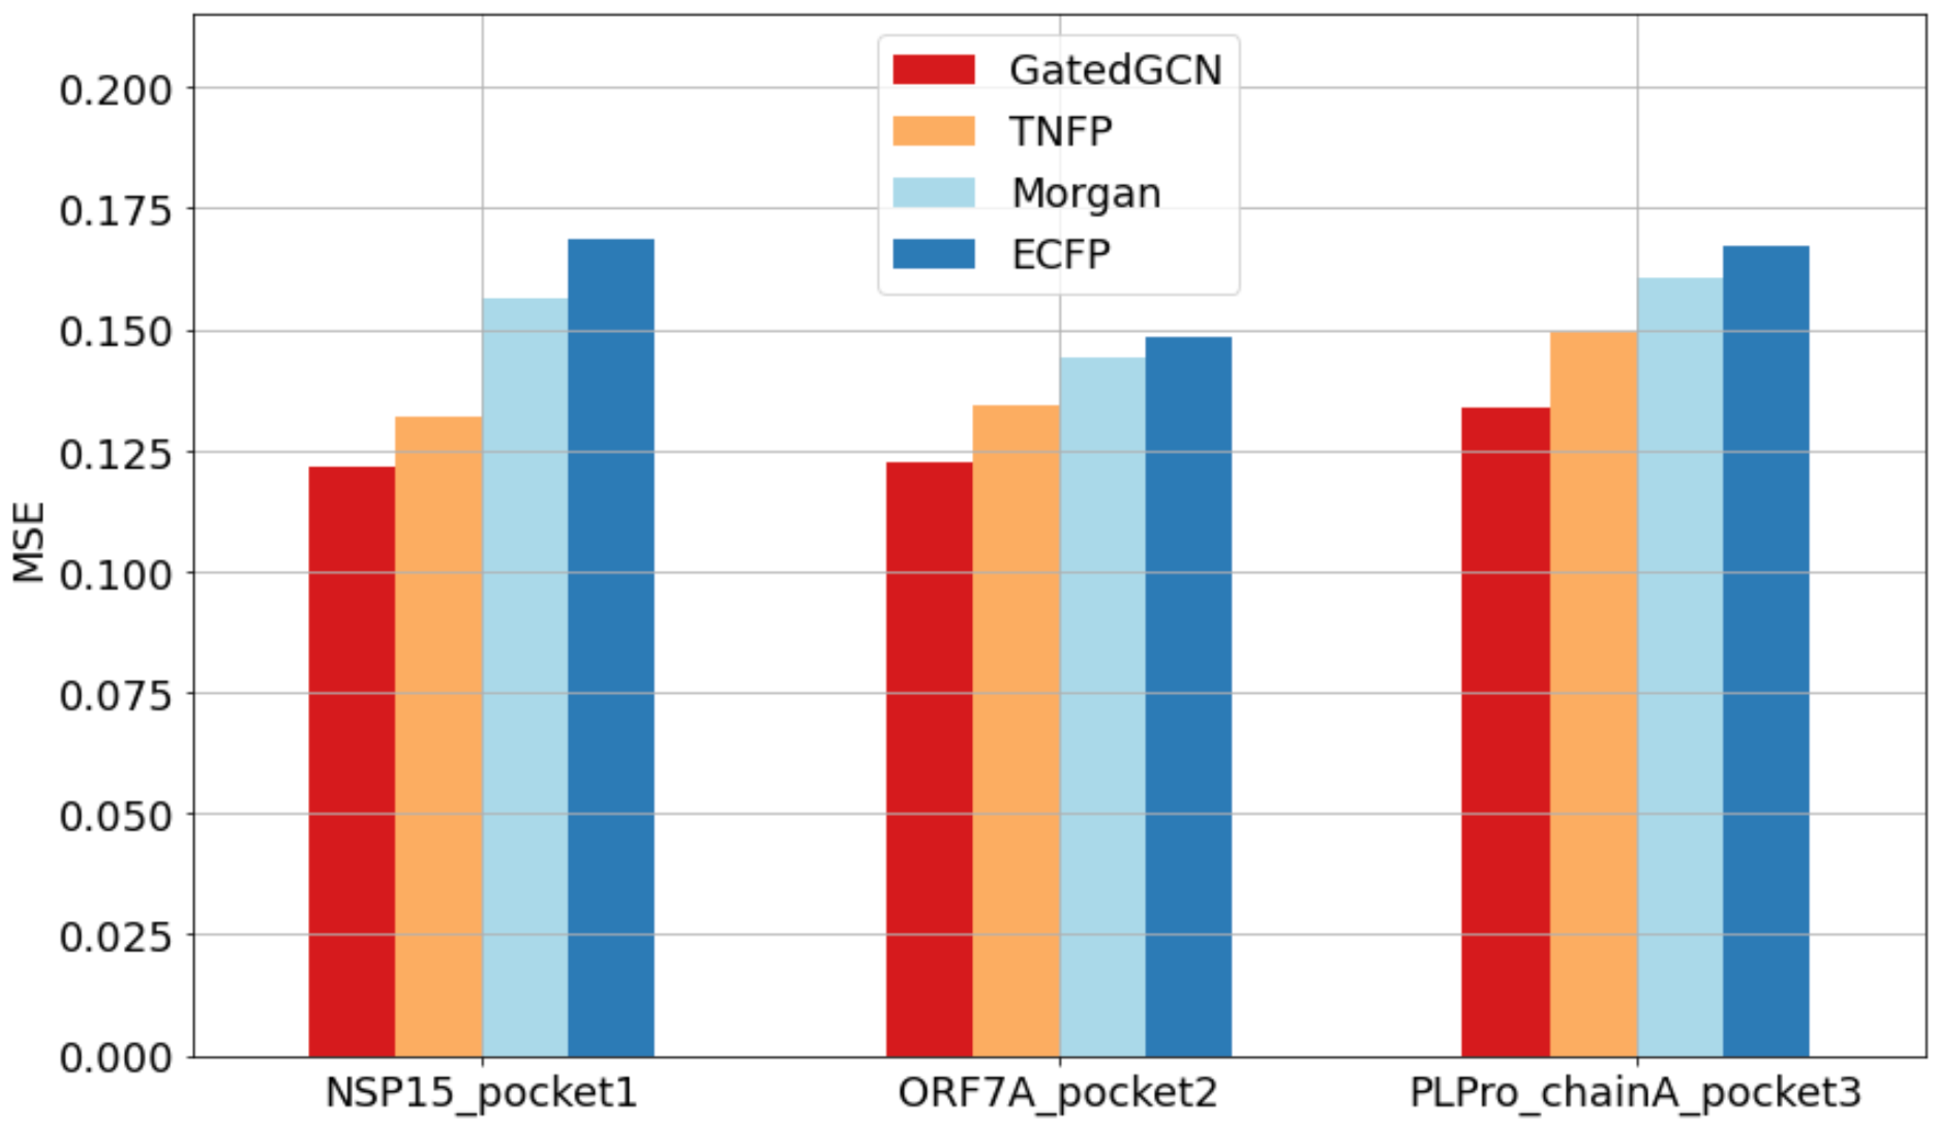
\includegraphics[width=0.9 \hsize]{FigS5_model_compare.pdf}
    \caption{\label{fig:comp_perf} Performance comparison of the TNFP model with the GatedGCN model (Fig.~2b) and two CFP models (Fig.~2a) tested on three targets. 
    }
\end{figure}

\begin{figure}[htb]
    \centering
    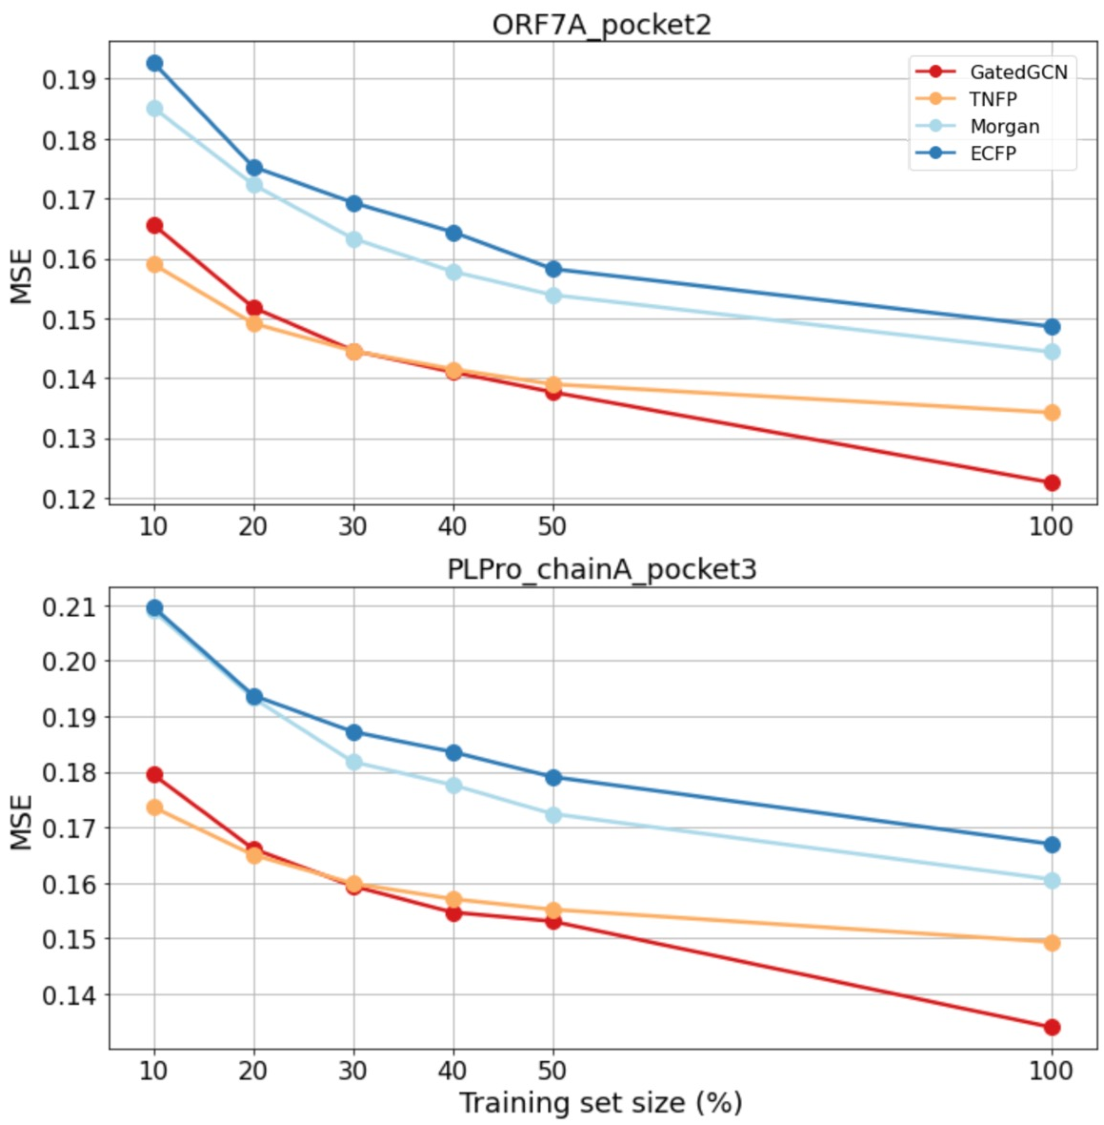
\includegraphics[width=0.9 \hsize]{FigS6_data_effi.pdf}
    \caption{\label{fig_s:data_eff} Training data efficiency of four different models shown for two test targets.
    }
\end{figure}

\clearpage
%\bibliography{gnn}
%merlin.mbs apsrev4-1.bst 2010-07-25 4.21a (PWD, AO, DPC) hacked
%Control: key (0)
%Control: author (72) initials jnrlst
%Control: editor formatted (1) identically to author
%Control: production of article title (-1) disabled
%Control: page (0) single
%Control: year (1) truncated
%Control: production of eprint (0) enabled
\begin{thebibliography}{2}%
\makeatletter
\providecommand \@ifxundefined [1]{%
 \@ifx{#1\undefined}
}%
\providecommand \@ifnum [1]{%
 \ifnum #1\expandafter \@firstoftwo
 \else \expandafter \@secondoftwo
 \fi
}%
\providecommand \@ifx [1]{%
 \ifx #1\expandafter \@firstoftwo
 \else \expandafter \@secondoftwo
 \fi
}%
\providecommand \natexlab [1]{#1}%
\providecommand \enquote  [1]{``#1''}%
\providecommand \bibnamefont  [1]{#1}%
\providecommand \bibfnamefont [1]{#1}%
\providecommand \citenamefont [1]{#1}%
\providecommand \href@noop [0]{\@secondoftwo}%
\providecommand \href [0]{\begingroup \@sanitize@url \@href}%
\providecommand \@href[1]{\@@startlink{#1}\@@href}%
\providecommand \@@href[1]{\endgroup#1\@@endlink}%
\providecommand \@sanitize@url [0]{\catcode `\\12\catcode `\$12\catcode
  `\&12\catcode `\#12\catcode `\^12\catcode `\_12\catcode `\%12\relax}%
\providecommand \@@startlink[1]{}%
\providecommand \@@endlink[0]{}%
\providecommand \url  [0]{\begingroup\@sanitize@url \@url }%
\providecommand \@url [1]{\endgroup\@href {#1}{\urlprefix }}%
\providecommand \urlprefix  [0]{URL }%
\providecommand \Eprint [0]{\href }%
\providecommand \doibase [0]{http://dx.doi.org/}%
\providecommand \selectlanguage [0]{\@gobble}%
\providecommand \bibinfo  [0]{\@secondoftwo}%
\providecommand \bibfield  [0]{\@secondoftwo}%
\providecommand \translation [1]{[#1]}%
\providecommand \BibitemOpen [0]{}%
\providecommand \bibitemStop [0]{}%
\providecommand \bibitemNoStop [0]{.\EOS\space}%
\providecommand \EOS [0]{\spacefactor3000\relax}%
\providecommand \BibitemShut  [1]{\csname bibitem#1\endcsname}%
\let\auto@bib@innerbib\@empty
%</preamble>
\bibitem [{\citenamefont {Harris}\ \emph {et~al.}(2020)\citenamefont {Harris},
  \citenamefont {Millman}, \citenamefont {van~der Walt}, \citenamefont
  {Gommers}, \citenamefont {Virtanen}, \citenamefont {Cournapeau},
  \citenamefont {Wieser}, \citenamefont {Taylor}, \citenamefont {Berg},
  \citenamefont {Smith} \emph {et~al.}}]{harris2020array}%
  \BibitemOpen
  \bibfield  {author} {\bibinfo {author} {\bibfnamefont {C.~R.}\ \bibnamefont
  {Harris}}, \bibinfo {author} {\bibfnamefont {K.~J.}\ \bibnamefont {Millman}},
  \bibinfo {author} {\bibfnamefont {S.~J.}\ \bibnamefont {van~der Walt}},
  \bibinfo {author} {\bibfnamefont {R.}~\bibnamefont {Gommers}}, \bibinfo
  {author} {\bibfnamefont {P.}~\bibnamefont {Virtanen}}, \bibinfo {author}
  {\bibfnamefont {D.}~\bibnamefont {Cournapeau}}, \bibinfo {author}
  {\bibfnamefont {E.}~\bibnamefont {Wieser}}, \bibinfo {author} {\bibfnamefont
  {J.}~\bibnamefont {Taylor}}, \bibinfo {author} {\bibfnamefont
  {S.}~\bibnamefont {Berg}}, \bibinfo {author} {\bibfnamefont {N.~J.}\
  \bibnamefont {Smith}},  \emph {et~al.},\ }\href@noop {} {\bibfield  {journal}
  {\bibinfo  {journal} {Nature}\ }\textbf {\bibinfo {volume} {585}},\ \bibinfo
  {pages} {357} (\bibinfo {year} {2020})}\BibitemShut {NoStop}%
\bibitem [{\citenamefont {Kingma}\ and\ \citenamefont
  {Ba}(2014)}]{kingma2014adam}%
  \BibitemOpen
  \bibfield  {author} {\bibinfo {author} {\bibfnamefont {D.~P.}\ \bibnamefont
  {Kingma}}\ and\ \bibinfo {author} {\bibfnamefont {J.}~\bibnamefont {Ba}},\
  }\href@noop {} {\bibfield  {journal} {\bibinfo  {journal} {arXiv:1412.6980}\
  } (\bibinfo {year} {2014})}\BibitemShut {NoStop}%
\end{thebibliography}%
\end{document}
